%!TEX TS-program = xelatex

% Шаблон документа LaTeX создан в 2018 году
% Алексеем Подчезерцевым
% В качестве исходных использованы шаблоны
% 	Данилом Фёдоровых (danil@fedorovykh.ru) 
%		https://www.writelatex.com/coursera/latex/5.2.2
%	LaTeX-шаблон для русской кандидатской диссертации и её автореферата.
%		https://github.com/AndreyAkinshin/Russian-Phd-LaTeX-Dissertation-Template

\documentclass[a4paper,14pt]{article}


%%% Работа с русским языком
\usepackage[english,russian]{babel}   %% загружает пакет многоязыковой вёрстки
\usepackage{fontspec}      %% подготавливает загрузку шрифтов Open Type, True Type и др.
\defaultfontfeatures{Ligatures={TeX},Renderer=Basic}  %% свойства шрифтов по умолчанию
\setmainfont[Ligatures={TeX,Historic}]{Times New Roman} %% задаёт основной шрифт документа
\setsansfont{Comic Sans MS}                    %% задаёт шрифт без засечек
\setmonofont{Courier New}
\usepackage{indentfirst}
\frenchspacing

\renewcommand{\epsilon}{\ensuremath{\varepsilon}}
\renewcommand{\phi}{\ensuremath{\varphi}}
\renewcommand{\kappa}{\ensuremath{\varkappa}}
\renewcommand{\le}{\ensuremath{\leqslant}}
\renewcommand{\leq}{\ensuremath{\leqslant}}
\renewcommand{\ge}{\ensuremath{\geqslant}}
\renewcommand{\geq}{\ensuremath{\geqslant}}
\renewcommand{\emptyset}{\varnothing}

%%% Дополнительная работа с математикой
\usepackage{amsmath,amsfonts,amssymb,amsthm,mathtools} % AMS
\usepackage{icomma} % "Умная" запятая: $0,2$ --- число, $0, 2$ --- перечисление

%% Номера формул
%\mathtoolsset{showonlyrefs=true} % Показывать номера только у тех формул, на которые есть \eqref{} в тексте.
%\usepackage{leqno} % Нумерация формул слева	

%% Перенос знаков в формулах (по Львовскому)
\newcommand*{\hm}[1]{#1\nobreak\discretionary{}
	{\hbox{$\mathsurround=0pt #1$}}{}}

%%% Работа с картинками
\usepackage{graphicx}  % Для вставки рисунков
\graphicspath{{images/}}  % папки с картинками
\setlength\fboxsep{3pt} % Отступ рамки \fbox{} от рисунка
\setlength\fboxrule{1pt} % Толщина линий рамки \fbox{}
\usepackage{wrapfig} % Обтекание рисунков текстом

%%% Работа с таблицами
\usepackage{array,tabularx,tabulary,booktabs} % Дополнительная работа с таблицами
\usepackage{longtable}  % Длинные таблицы
\usepackage{multirow} % Слияние строк в таблице
\usepackage{float}% http://ctan.org/pkg/float

%%% Программирование
\usepackage{etoolbox} % логические операторы


%%% Страница
\usepackage{extsizes} % Возможность сделать 14-й шрифт
\usepackage{geometry} % Простой способ задавать поля
\geometry{top=20mm}
\geometry{bottom=20mm}
\geometry{left=20mm}
\geometry{right=10mm}
%
%\usepackage{fancyhdr} % Колонтитулы
% 	\pagestyle{fancy}
%\renewcommand{\headrulewidth}{0pt}  % Толщина линейки, отчеркивающей верхний колонтитул
% 	\lfoot{Нижний левый}
% 	\rfoot{Нижний правый}
% 	\rhead{Верхний правый}
% 	\chead{Верхний в центре}
% 	\lhead{Верхний левый}
%	\cfoot{Нижний в центре} % По умолчанию здесь номер страницы

\usepackage{setspace} % Интерлиньяж
\onehalfspacing % Интерлиньяж 1.5
%\doublespacing % Интерлиньяж 2
%\singlespacing % Интерлиньяж 1

\usepackage{lastpage} % Узнать, сколько всего страниц в документе.

\usepackage{soul} % Модификаторы начертания

\usepackage{hyperref}
\usepackage[usenames,dvipsnames,svgnames,table,rgb]{xcolor}
\hypersetup{				% Гиперссылки
	unicode=true,           % русские буквы в раздела PDF
	pdftitle={Заголовок},   % Заголовок
	pdfauthor={Автор},      % Автор
	pdfsubject={Тема},      % Тема
	pdfcreator={Создатель}, % Создатель
	pdfproducer={Производитель}, % Производитель
	pdfkeywords={keyword1} {key2} {key3}, % Ключевые слова
	colorlinks=true,       	% false: ссылки в рамках; true: цветные ссылки
	linkcolor=black,          % внутренние ссылки
	citecolor=black,        % на библиографию
	filecolor=magenta,      % на файлы
	urlcolor=black           % на URL
}
\makeatletter 
\def\@biblabel#1{#1. } 
\makeatother
\usepackage{cite} % Работа с библиографией
%\usepackage[superscript]{cite} % Ссылки в верхних индексах
%\usepackage[nocompress]{cite} % 
\usepackage{csquotes} % Еще инструменты для ссылок

\usepackage{multicol} % Несколько колонок

\usepackage{tikz} % Работа с графикой
\usepackage{pgfplots}
\usepackage{pgfplotstable}

% ГОСТ заголовки
\usepackage[font=small]{caption}
%\captionsetup[table]{justification=centering, labelsep = newline} % Таблицы по правобу краю
%\captionsetup[figure]{justification=centering} % Картинки по центру


\newcommand{\tablecaption}[1]{\addtocounter{table}{1}\small \begin{flushright}\tablename \ \thetable\end{flushright}%	
\begin{center}#1\end{center}}

\newcommand{\imref}[1]{рис.~\ref{#1}}

\usepackage{multirow}
\usepackage{spreadtab}
\newcolumntype{K}[1]{@{}>{\centering\arraybackslash}p{#1cm}@{}}


\usepackage{xparse}
\usepackage{fancyvrb}

\RecustomVerbatimCommand{\VerbatimInput}{VerbatimInput}
{
	fontsize=\footnotesize    
}

\usepackage{tocloft}
\renewcommand{\cftsecleader}{\cftdotfill{\cftdotsep}}
\begin{document} % конец преамбулы, начало документа
\begin{titlepage}
	\begin{center}
 		ФЕДЕРАЛЬНОЕ  ГОСУДАРСТВЕННОЕ АВТОНОМНОЕ \\
		ОБРАЗОВАТЕЛЬНОЕ УЧРЕЖДЕНИЕ ВЫСШЕГО ОБРАЗОВАНИЯ\\
		«НАЦИОНАЛЬНЫЙ ИССЛЕДОВАТЕЛЬСКИЙ УНИВЕРСИТЕТ\\
		«ВЫСШАЯ ШКОЛА ЭКОНОМИКИ»
	\end{center}
	
	\begin{center}
		\textbf{Московский институт электроники и математики}
		
		\textbf{им. А.Н.Тихонова НИУ ВШЭ}
		
		\vspace{2ex}
		
		\textbf{Департамент компьютерной инженерии}
	\end{center}
	\vspace{1ex}	
	
	\begin{center}
	\textbf{ОТЧЕТ\\
		ПО ЛАБОРАТОРНОЙ РАБОТЕ №6
	}
	\end{center}	
	\vspace{2ex}
	\begin{center}
		по дисциплине «Проектирование систем на кристалле»
	\end{center}	

	\vspace{2ex}

	\begin{flushright}
		\textbf{Выполнили:}
		
		\vspace{2ex}
		
		Студенты группы БИВ174
		
		Бригада №5
		
		\vspace{2ex}
		
		Подчезерцев Алексей Евгеньевич
		
		Солодянкин Андрей Александрович
		\vspace{2ex}
		
	\end{flushright}

	\vfill
	\begin{center}
		Москва \the\year \, г.
	\end{center}
	
\end{titlepage}
\addtocounter{page}{1}
\tableofcontents
\pagebreak
\section{Задание}

\begin{enumerate}
	\item Исследуйте работу и проведите моделирование еще одной версии однобитного
	мультиплексора, реализованного с помощью операции конкатенации.
	
	\item Синтезируйте вышеупомянутые реализации мультиплексоров в Quartus Prime. Рассмотрите
	их представление в RTL Viewer, объясните, в чем состоит ошибка в модуле
	b2\_mux\_2\_1\_comb\_incorrect (Листинг 4.8).
	
	\item Проанализируйте полученные в Quartus Prime RТL-схемы мультиплексоров 4в1. Объясните,	какая реализация, по Вашему мнению, является наиболее быстрой; какая занимает меньше всего пространства на чипе; какой подход проще всего масштабировать.
	
	\item Разработайте мультиплексор Звl с использованием оператора if, чтобы он был реализован с	помощью регистра защелки, а затем исправьте его, удалив регистр защелки. Представьте	результаты моделирования и синтеза в RTL и объясните их. Загрузите результаты в Technology map viewer и дайте пояснения тому, что получится.
	
	\item Изучите примеры в книге «Цифровая схемотехника и архитектура компьютера», после чего	разработайте таблицу истинности и изобразите условную схему подключения мультиплексора 4в1, который реализует логический элемент исключающее ИЛИ. Опишите	логическую функцию $y = (\bar A \wedge B \wedge C) \vee (A \wedge \bar B \wedge \bar C)$ с помощью мультиплексора 8в1.
	
	\item Измените значение параметра $DATA\_WIDTH$ в модуле демультиплексора на значения 4, 8, 16, 32, 64, 128. Оцените изменение потребляемых ресурсов после синтеза, опишите и объясните полученные зависимости.
	
	\item Предложите другой вариант селектора, синтезируйте его и проведите моделирование. Сравните свою реализацию с предлагаемой в данном мануале.
	
	\item Ответьте на вопрос, почему нельзя модуль полностью параметризированного мультиплексора (Листинг 4.23) реализовать по аналогии с селектором (Листинг 4.24) следующим образом: $assign у= data[((sel+l)*DATA\_WIDTH) - 1: (sel*DATA\_WIDTH)]$;
	
\end{enumerate}

\section{Дополнительные задания}

\subsection{1 задание}
 
 Исследуйте работу и проведите моделирование еще одной версии однобитного
мультиплексора, реализованного с помощью операции конкатенации.

\VerbatimInput{../z1/b1_mux_2_1_concate.v}

\begin{figure}[H]
	\centering
	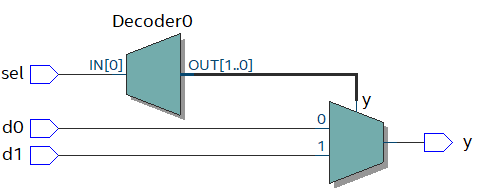
\includegraphics[width=0.6\linewidth]{img/z1_rtl}
	\caption{RTL представление однобитного
		мультиплексора на операции конкатенации}
	\label{fig:z1_rtl}
\end{figure}

\begin{figure}[H]
	\centering
	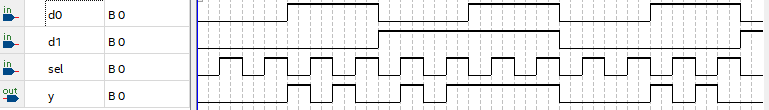
\includegraphics[width=0.75\linewidth]{img/z1_wvf}
	\caption{WVF однобитного мультиплексора на операции конкатенации}
	\label{fig:z1_wvf}
\end{figure}

\subsection{2 задание}

Синтезируйте вышеупомянутые реализации мультиплексоров в Quartus Prime. Рассмотрите их представление в RTL Viewer, объясните, в чем состоит ошибка в модуле b2\_mux\_2\_1\_comb\_incorrect (Листинг 4.8).

\VerbatimInput{../z1/b2_mux_2_1_sel.v} 

\begin{figure}[H]
	\centering
	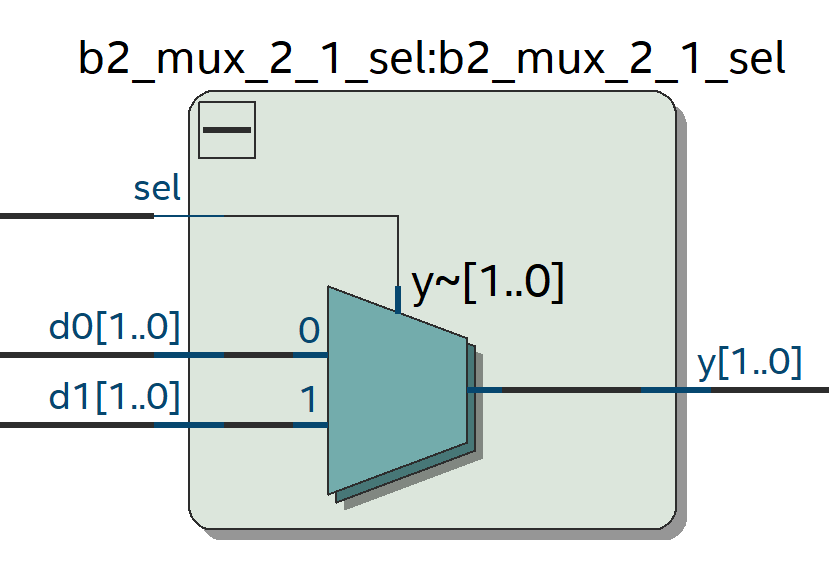
\includegraphics[width=0.6\linewidth]{img/z2_rtl_sel}
	\caption{RTL представление двухбитного мультиплексора на основе тернарного оператора}
	\label{fig:z2_rtl_sel}
\end{figure}

\VerbatimInput{../z1/b2_mux_2_1_if.v} 

\begin{figure}[H]
	\centering
	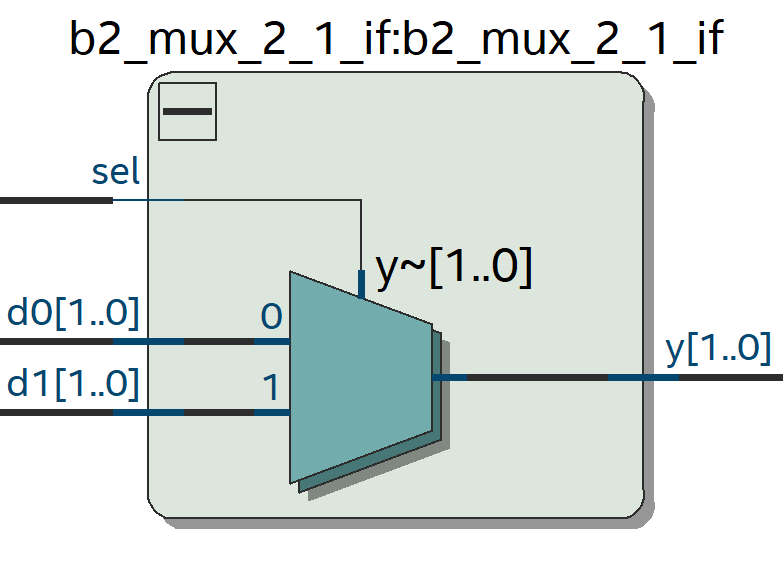
\includegraphics[width=0.6\linewidth]{img/z2_rtl_if}
	\caption{RTL представление двухбитного
		мультиплексора на операции if}
	\label{fig:z2_rtl_if}
\end{figure}


\VerbatimInput{../z1/b2_mux_2_1_comb_correct1.v} 

\begin{figure}[H]
	\centering
	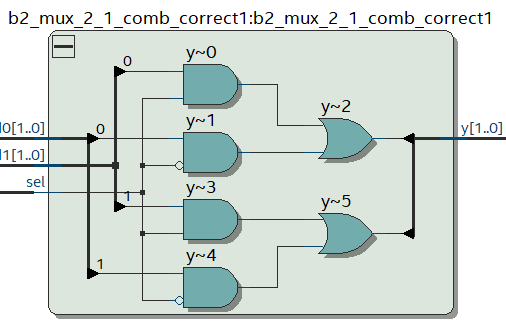
\includegraphics[width=0.6\linewidth]{img/z2_rtl_cor1}
	\caption{RTL представление двухбитного комбинационного мультиплексора 1}
	\label{fig:z2_rtl_cor1}
\end{figure}
	

\VerbatimInput{../z1/b2_mux_2_1_comb_correct2.v} 

\begin{figure}[H]
	\centering
	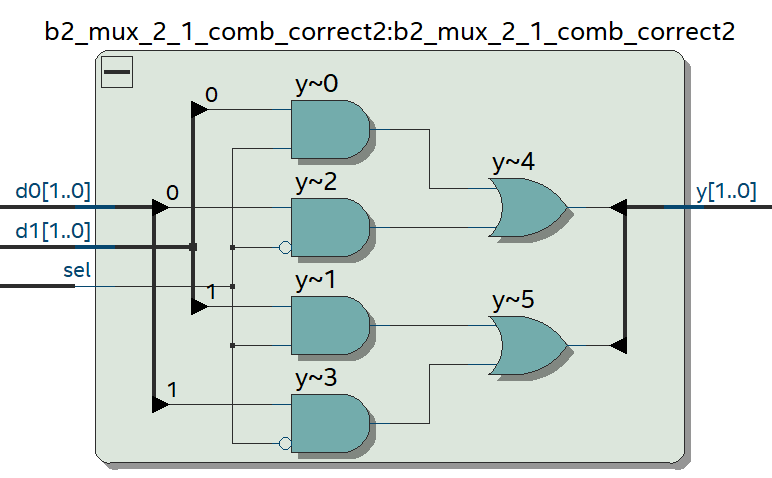
\includegraphics[width=0.6\linewidth]{img/z2_rtl_cor2}
	\caption{RTL представление двухбитного комбинационного мультиплексора 2}
	\label{fig:z2_rtl_cor2}
\end{figure}


\VerbatimInput{../z1/b2_mux_2_1_comb_incorrect.v} 

В данном примере используются побитовые операции, в связи с чем
надо следить за размерностью участвующих в них операндов. Размер операнда $sel$ равен 1, размеры входных операндов $d[0],d[1]$ равны 2. Для корректной работы необходимо обращаться к каждому биту в $d[0],d[1]$ или перевести $sel$ к длине операндов $d[0],d[1]$.

\subsection{3 задание}

Проанализируйте полученные в Quartus Prime RТL-схемы мультиплексоров 4в1. Объясните, какая реализация, по Вашему мнению, является наиболее быстрой;  какая занимает меньше всего пространства на чипе; какой подход проще всего масштабировать.

\VerbatimInput{../z1/b2_mux_4_1_sel.v} 

\begin{figure}[H]
 	\centering
 	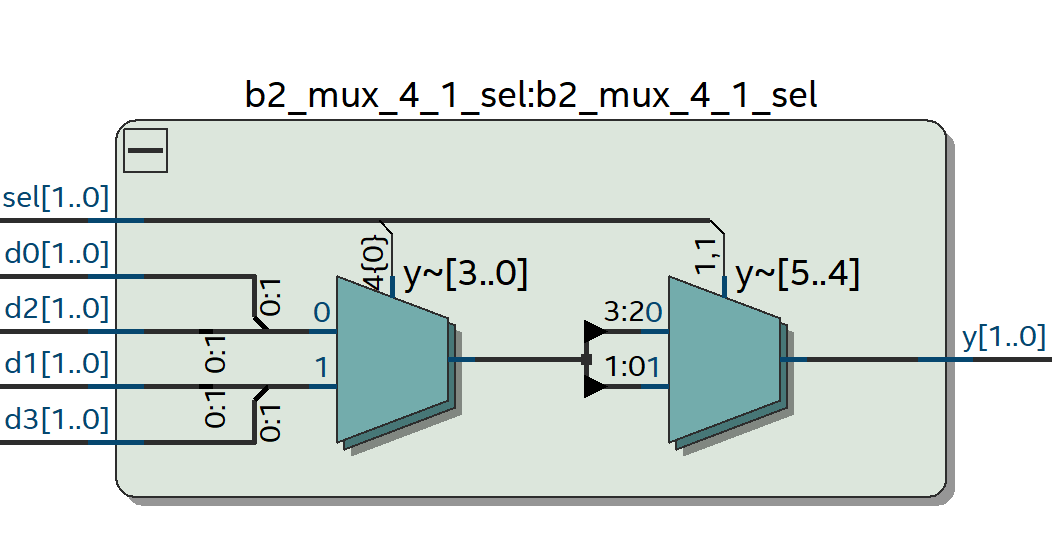
\includegraphics[width=0.6\linewidth]{img/z3_rtl_sel}
 	\caption{RTL представление двухбитного мультиплексора на основе тернарного оператора}
 	\label{fig:z3_rtl_sel}
\end{figure}

\VerbatimInput{../z1/b2_mux_4_1_case.v} 

\begin{figure}[H]
	\centering
	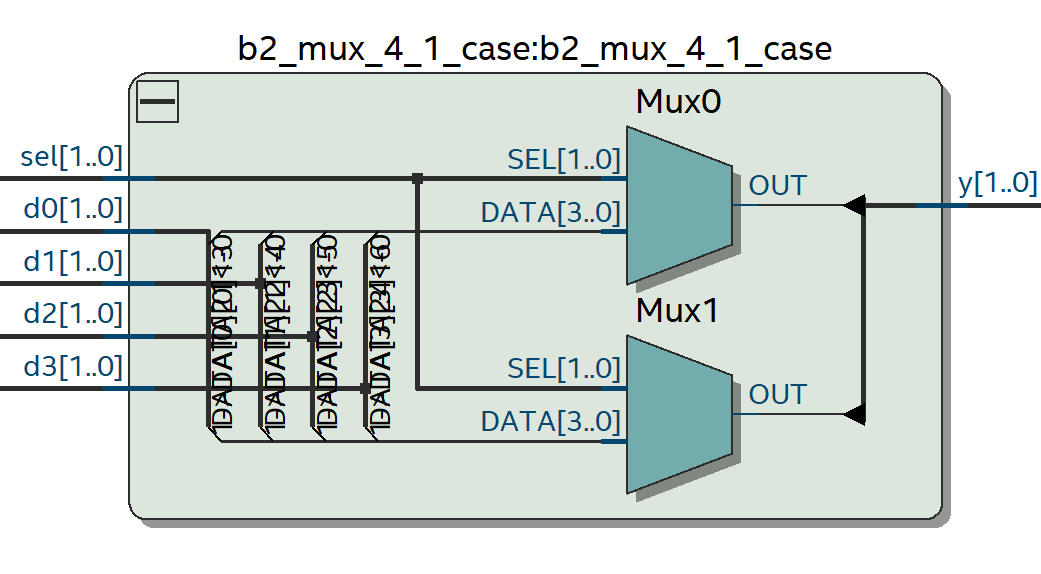
\includegraphics[width=0.6\linewidth]{img/z3_rtl_case}
	\caption{RTL представление двухбитного мультиплексора на операторе case}
	\label{fig:z3_rtl_case}
\end{figure}


\VerbatimInput{../z1/b2_mux_4_1_block.v} 

\begin{figure}[H]
	\centering
	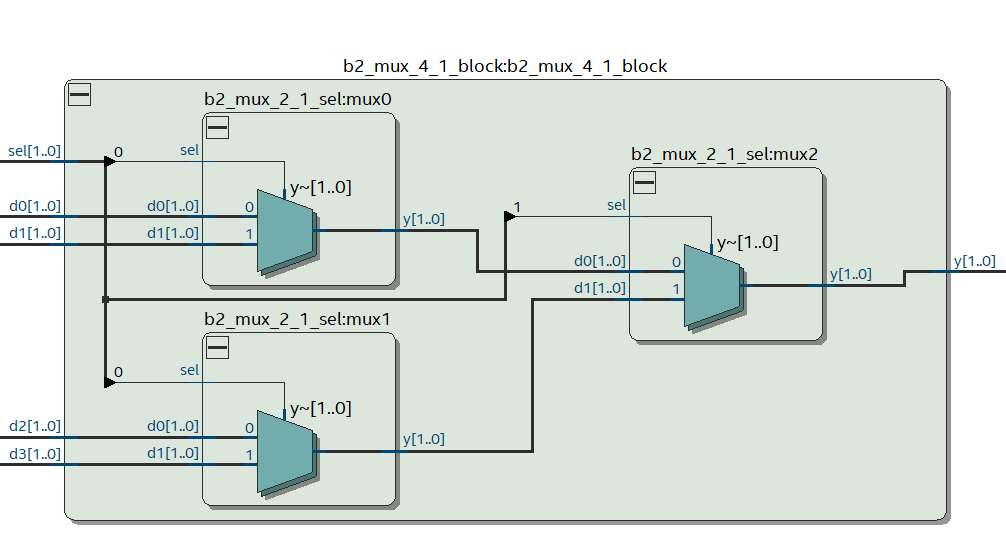
\includegraphics[width=0.6\linewidth]{img/z3_rtl_block}
	\caption{RTL представление двухбитного модульного мультиплексора }
	\label{fig:z3_rtl_block}
\end{figure}

\VerbatimInput{../z1/b2_mux_4_1_block_alt.v} 

\begin{figure}[H]
	\centering
	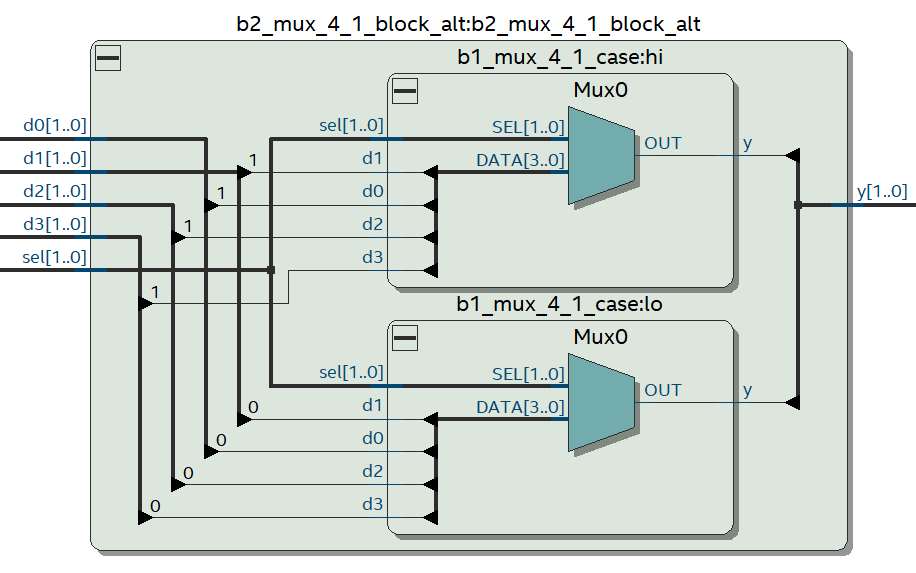
\includegraphics[width=0.6\linewidth]{img/z3_rtl_block_alt}
	\caption{RTL представление двухбитного альтернативно модульного мультиплексора}
	\label{fig:z3_rtl_block_alt}
\end{figure}

Меньше всего пространства на чипе занимает мультиплексор на тернарном операторе.

Самыми быстродействующими являются мультиплексор на операторе case и альтернативный модульный мультиплексор, в них по 2 параллельных мультиплексора.

Лучше всего масштабируется по количеству информационных входов модульный мультиплексор.

Лучше всего масштабируется по длине информационного сигнала альтернативный модульный мультиплексор.

\subsection{4 задание}

Разработайте мультиплексор Звl с использованием оператора if, чтобы он был реализован с помощью регистра защелки, а затем исправьте его, удалив регистр защелки. Представьте результаты моделирования и синтеза в RTL и объясните их. Загрузите результаты в Technology map viewer и дайте пояснения тому, что получится.

\VerbatimInput{../z1/b2_mux_3_1_if_latch.v} 

\begin{figure}[H]
	\centering
	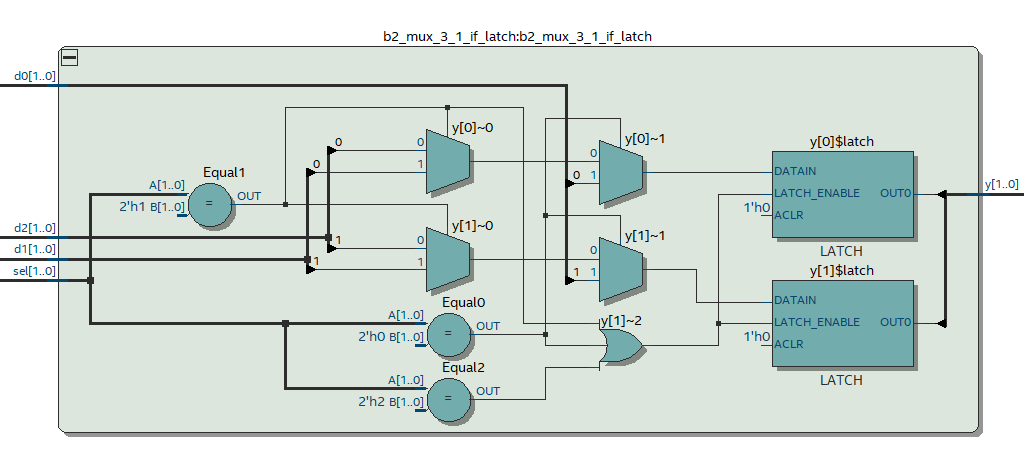
\includegraphics[width=0.6\linewidth]{img/z4_rtl_if_latch}
	\caption{RTL представление неполного мультиплексора с защелкой}
	\label{fig:z4_rtl_if_latch}
\end{figure}

\begin{figure}[H]
	\centering
	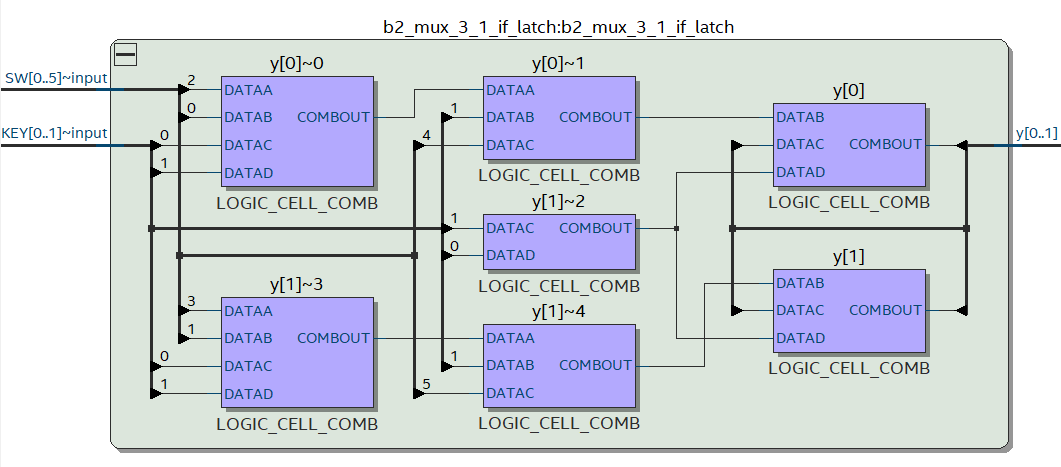
\includegraphics[width=0.6\linewidth]{img/z4_tmv_if_latch}
	\caption{Результаты в Technology map viewer неполного мультиплексора с защелкой}
	\label{fig:z4_tmv_if_latch}
\end{figure}

\VerbatimInput{../z1/b2_mux_3_1_if_correct.v} 

\begin{figure}[H]
	\centering
	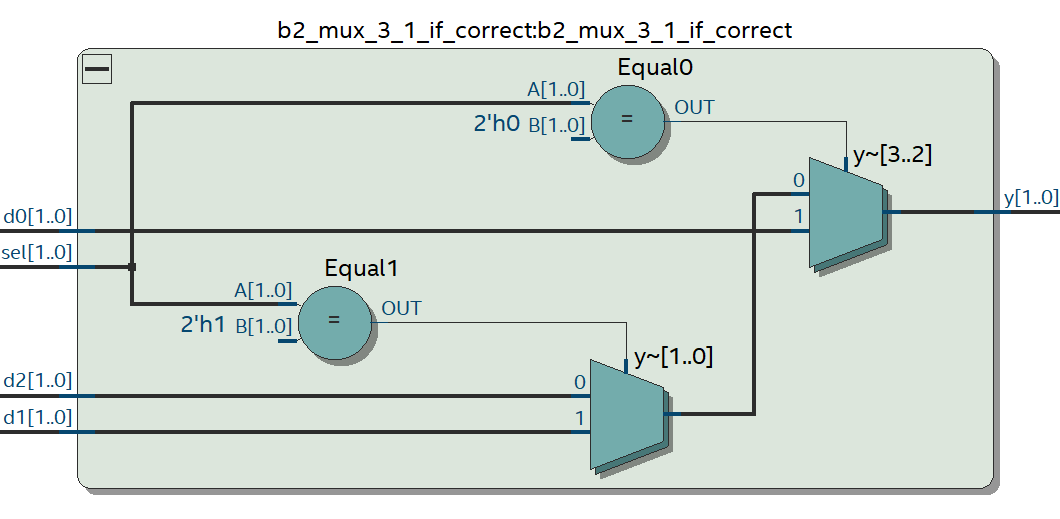
\includegraphics[width=0.6\linewidth]{img/z4_rtl_if_correct}
	\caption{RTL представление неполного мультиплексора с дефолтным значением}
	\label{fig:z4_rtl_if_correct}
\end{figure}

\begin{figure}[H]
	\centering
	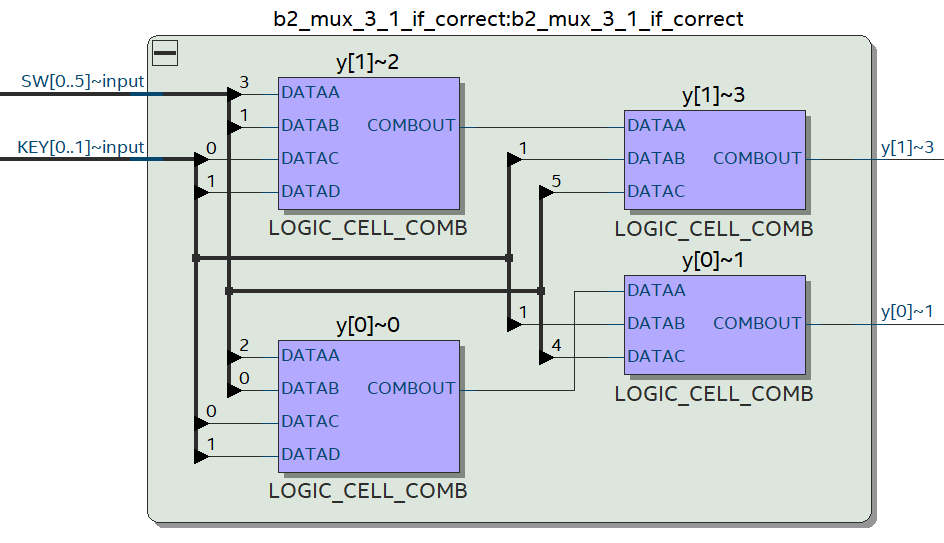
\includegraphics[width=0.6\linewidth]{img/z4_tmv_if_correct}
	\caption{Результаты в Technology map viewer неполного мультиплексора с дефолтным значением}
	\label{fig:z4_tmv_if_correct}
\end{figure}

\VerbatimInput{../z1/b2_mux_3_1_ifx_correct.v} 

\begin{figure}[H]
	\centering
	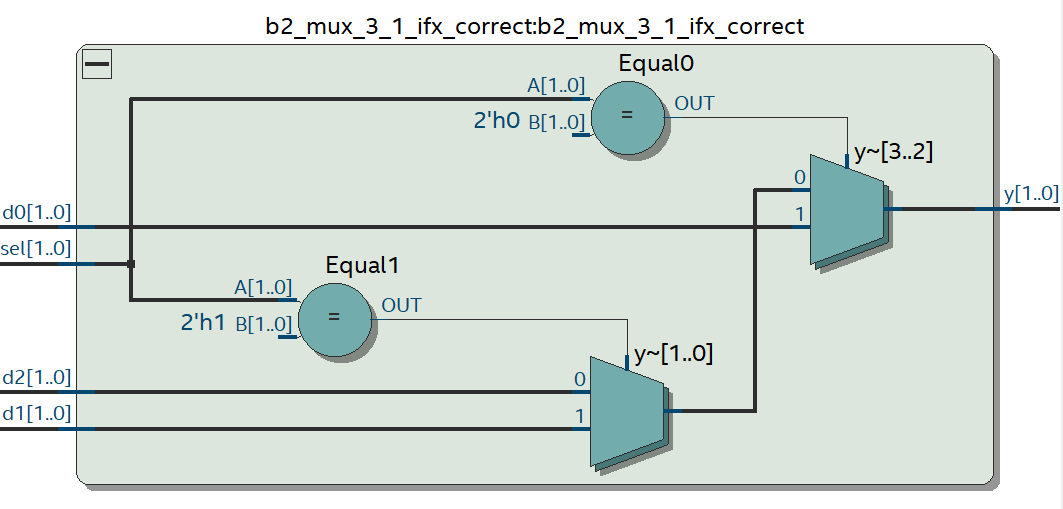
\includegraphics[width=0.6\linewidth]{img/z4_rtl_ifx_correct}
	\caption{RTL представление неполного мультиплексора с неопределенным значением}
	\label{fig:z4_rtl_ifx_correct}
\end{figure}

\begin{figure}[H]
	\centering
	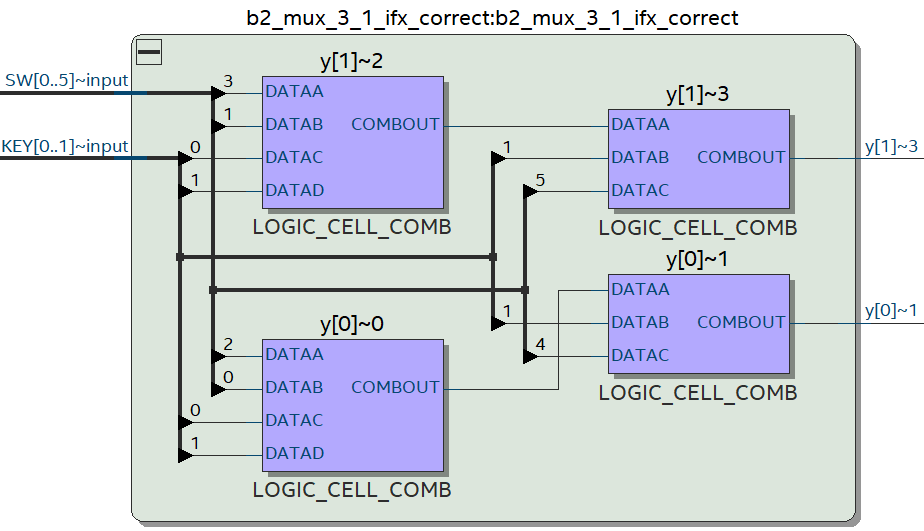
\includegraphics[width=0.6\linewidth]{img/z4_tmv_ifx_correct}
	\caption{Результаты в Technology map viewer неполного мультиплексора с неопределенным значением}
	\label{fig:z4_tmv_ifx_correct}
\end{figure}

\subsection{5 задание}

Изучите примеры в книге «Цифровая схемотехника и архитектура компьютера», после чего	разработайте таблицу истинности и изобразите условную схему подключения мультиплексора 4в1, который реализует логический элемент исключающее ИЛИ. 

\begin{table}[H]
	\begin{center}
		\begin{flushleft}
			\tablecaption{Таблица истинности для исключающего ИЛИ}
		\end{flushleft}
		\label{tab:iskl_ili}
		\begin{tabular}{|c|c|c|}
			\hline
			X1 & X2 & Y \\ \hline
			0  & 0  & 0 \\ \hline
			0  & 1  & 1 \\ \hline
			1  & 0  & 1 \\ \hline
			1  & 1  & 0 \\ \hline
		\end{tabular}
	\end{center}
\end{table}

\begin{figure}[H]
	\centering
	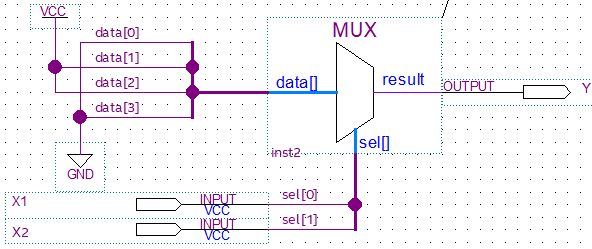
\includegraphics[width=0.6\linewidth]{img/z5_sh_iskl_ili}
	\caption{Условная схема подключения мультиплексора 4в1}
	\label{fig:z5_sh_iskl_ili}
\end{figure}

Опишите логическую функцию $y = (\bar A \wedge B \wedge C) \vee (A \wedge \bar B \wedge \bar C)$ с помощью мультиплексора 8в1.

\begin{table}[H]
	\begin{center}
		\begin{flushleft}
			\tablecaption{Таблица истинности для функции $y = (\bar A \wedge B \wedge C) \vee (A \wedge \bar B \wedge \bar C)$ }
		\end{flushleft}
		\label{tab:func}
		\begin{tabular}{|c|c|c|c|}
			\hline
			A & B & C & Y \\ \hline
			0 & 0 & 0 & 0 \\ \hline
			0 & 0 & 1 & 0 \\ \hline
			0 & 1 & 0 & 0 \\ \hline
			0 & 1 & 1 & 1 \\ \hline
			1 & 0 & 0 & 1 \\ \hline
			1 & 0 & 1 & 0 \\ \hline
			1 & 1 & 0 & 0 \\ \hline
			1 & 1 & 1 & 0 \\ \hline
		\end{tabular}
	\end{center}
\end{table}


\VerbatimInput{../z1/b1_func_8_1_case.v} 

\begin{figure}[H]
	\centering
	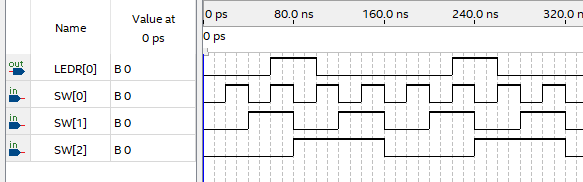
\includegraphics[width=0.6\linewidth]{img/z5_wvf_b8}
	\caption{WVF для функции $y = (\bar A \wedge B \wedge C) \vee (A \wedge \bar B \wedge \bar C)$}
	\label{fig:z5_wvf_b8}
\end{figure}

\subsection{6 задание}

Измените значение параметра $DATA\_WIDTH$ в модуле демультиплексора на значения 4, 8, 16, 32, 64, 128. Оцените изменение потребляемых ресурсов после синтеза, опишите и объясните полученные зависимости.

\VerbatimInput{../z1/bn_demux_1_4_case.v}

\begin{figure}[H]
	\centering
	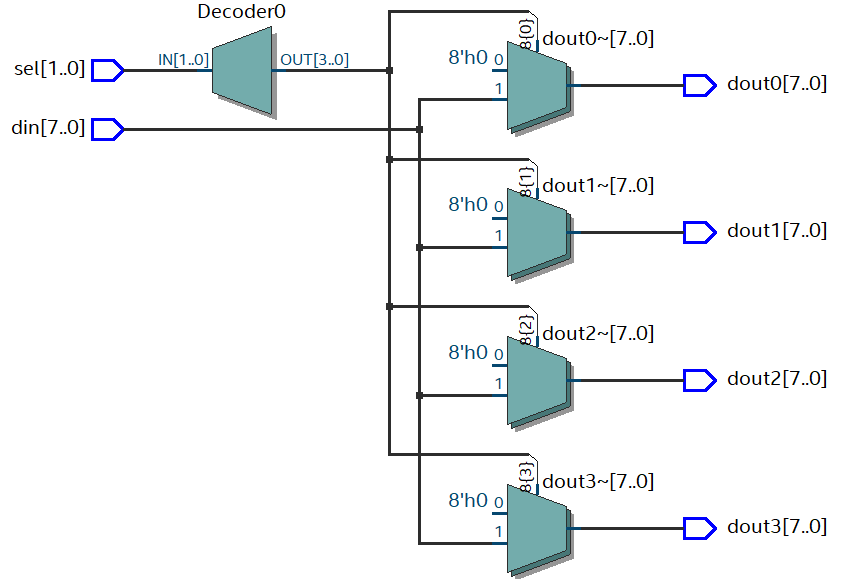
\includegraphics[width=0.6\linewidth]{img/z6_sh}
	\caption{RTL представление модуля демультиплексора}
	\label{fig:z6_sh}
\end{figure}

\begin{table}[H]
	\begin{center}
		\begin{flushleft}
			\tablecaption{Потребление ресурсов для различной длины  параметра $DATA\_WIDTH$}
		\end{flushleft}
		\label{tab:mnogo}
		\begin{tabular}{|c|c|c|}
			\hline
			DATA\_WIDTH & \begin{tabular}[c]{@{}c@{}}количество\\ логических\\ элементов\end{tabular} & \begin{tabular}[c]{@{}c@{}}количество\\ пинов\end{tabular} \\ \hline
			4           & 17                                                                          & 22                                                         \\ \hline
			8           & 33                                                                          & 42                                                         \\ \hline
			16          & 65                                                                          & 82                                                         \\ \hline
			32          & 129                                                                         & 162                                                        \\ \hline
			64          & 257                                                                         & 322                                                        \\ \hline
		\end{tabular}
	\end{center}
\end{table}

Для $DATA\_WIDTH = 128$ не удалось скомпилировать программу, т.к. максимальное количество пинов на схеме равно 360, а требовалось 642. Однако по полученным данным можно выявить зависимость числа логических элементов и пинов от $DATA\_WIDTH$.

Количество логических элементов можно вычислить по формуле \ref{eq:log}.

\begin{equation}
N_{log} = DATA\_WIDTH * m + 1
\label{eq:log}
\end{equation}

Где $N_{log}$ -- количество логических элементов, $m$ -- количество информационных сигналов на входе. Оставшийся 1 элемент это декодер.

Количество пинов можно вычислить по формуле \ref{eq:pins}.

\begin{equation}
N_{pin} = DATA\_WIDTH * (m + n) + k
\label{eq:pins}
\end{equation}

Где $N_{pin}$ -- количество пинов, $m$ -- количество информационных сигналов на входе, $n$ -- количество информационных сигналов на выходе, $k$ -- количество управляющих пинов

\subsection{7 задание}

Предложите другой вариант селектора, синтезируйте его и проведите моделирование. Сравните свою реализацию с предлагаемой в данном мануале.

Реализация селектора из мануала:

\VerbatimInput{../z1/bn_select_8_1_case.v}

\begin{figure}[H]
	\centering
	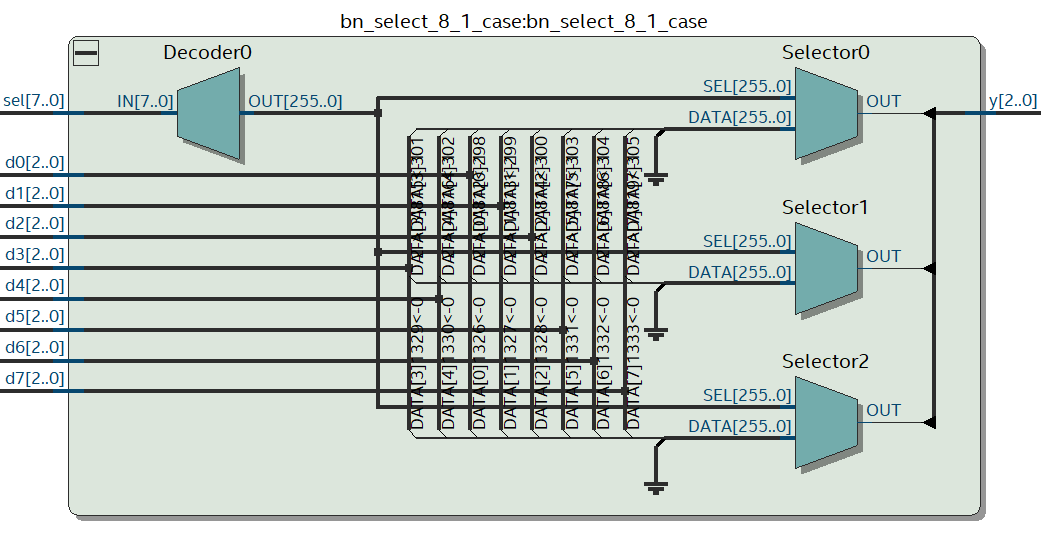
\includegraphics[width=0.6\linewidth]{img/z7_rtl_case}
	\caption{RTL представление селектора на операторе case}
	\label{fig:z7_rtl_case}
\end{figure}

Своя реализация селектора:

\VerbatimInput{../z1/bn_select_8_1_comb.v}

\begin{figure}[H]
	\centering
	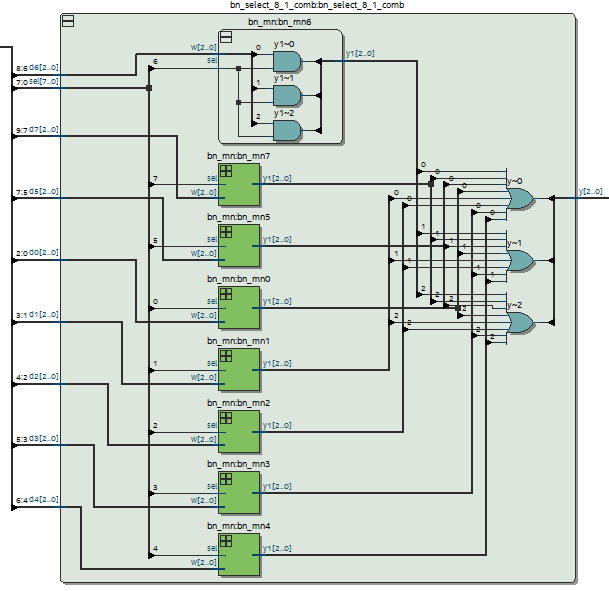
\includegraphics[width=0.7\linewidth]{img/z7_rtl_comb}
	\caption{RTL представление комбинационного селектора}
	\label{fig:z7_rtl_comb}
\end{figure}

\subsection{8 задание}

Ответьте на вопрос, почему нельзя модуль полностью параметризированного мультиплексора (Листинг 4.23) реализовать по аналогии с селектором (Листинг 4.24) следующим образом: $assign у= data[((sel+l)*DATA\_WIDTH) - 1: (sel*DATA\_WIDTH)]$;

Это сделать невозможно, ввиду того, что у мультиплексора и селектора разные управляющие сигналы. В селектор сигнал поступает уже декодированный, т.е. в унитарном виде. В мультиплексор управляющий сигнал подается в двоичном виде.

\section{Задания для самостоятельной работы}

\subsection{1 задание}

Используя примеры кода из данной главы, реализуйте следующие
мультиплексоры:

6. Мультиплексор 8в1, создав два мультиплексора 4в1 и один мультиплексор 2в1.
Реализовать модули мультиплексоров 4в1 и 2в1, используя оператор case.

\VerbatimInput{../z1/b2_mux_2_1_case.v}

\VerbatimInput{../z1/b2_mux_4_1_case.v}

\VerbatimInput{../z1/b2_mux_8_1_block.v}

\begin{figure}[H]
	\centering
	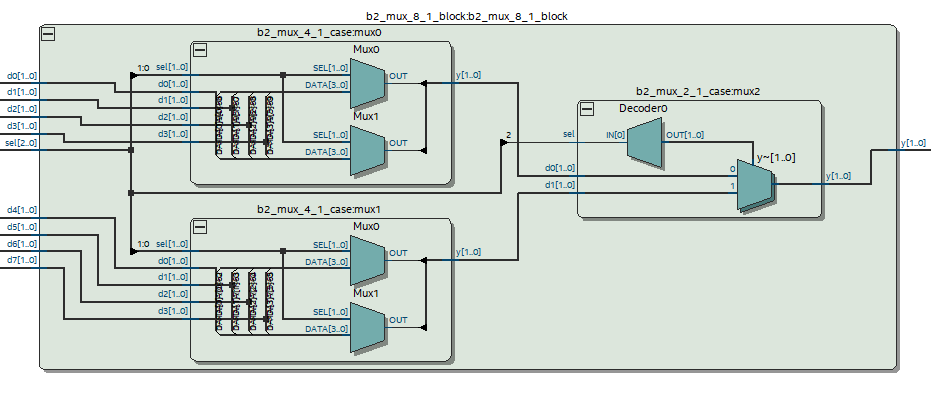
\includegraphics[width=0.6\linewidth]{img/dop1_rtl}
	\caption{RTL представление мультиплексора 8в1}
	\label{fig:dop1_rtl}
\end{figure}

\begin{figure}[H]
	\centering
	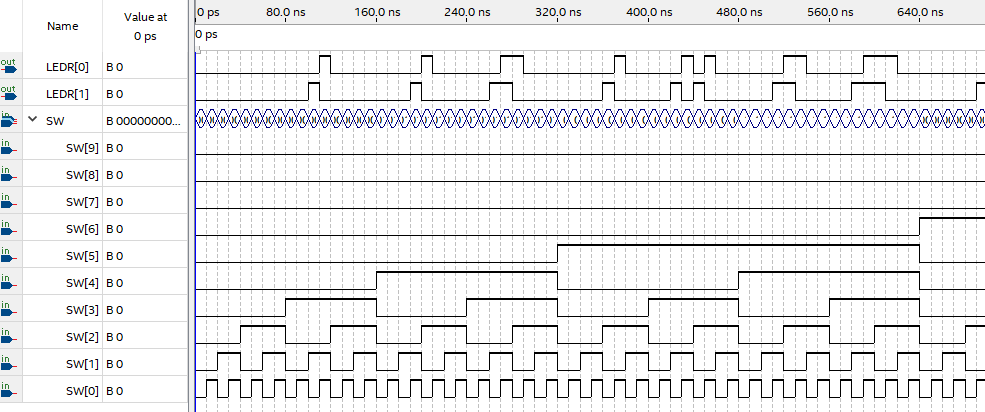
\includegraphics[width=0.6\linewidth]{img/dop1_wvf}
	\caption{WVF  мультиплексора 8в1}
	\label{fig:dop1_wvf}
\end{figure}
  
\subsection{2 задание}

Разработайте таблицу истинности и изобразите условную схему
подключения:

1. Мультиплексора 4в1, который реализует логический элемент ИЛИ-НЕ.

\begin{table}[H]
	\begin{center}
		\begin{flushleft}
			\tablecaption{Таблица истинности для ИЛИ-НЕ}
		\end{flushleft}
		\label{tab:ili_ne}
		\begin{tabular}{|c|c|c|}
			\hline
			X1 & X2 & Y \\ \hline
			0  & 0  & 1 \\ \hline
			0  & 1  & 0 \\ \hline
			1  & 0  & 0 \\ \hline
			1  & 1  & 0 \\ \hline
		\end{tabular}
	\end{center}
\end{table}

\begin{figure}[H]
	\centering
	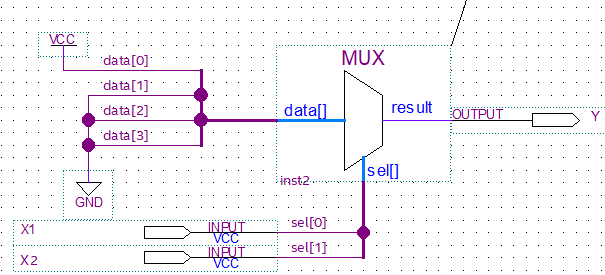
\includegraphics[width=0.6\linewidth]{img/dop2_sh}
	\caption{Условная схема подключения мультиплексора 4в1 ИЛИ-НЕ}
	\label{fig:dop2_sh}
\end{figure}

\subsection{3 задание}

С помощью мультиплексора 8в1 опишите логическую функцию в виде
условной схемы подключения: 

\begin{equation}
y = (A \vee B \vee C) \wedge (A \vee \bar B \vee \bar C) \wedge ( \bar A \vee \bar B \vee \bar C)
\label{eq:zad}
\end{equation}

\begin{table}[H]
	\begin{center}
		\begin{flushleft}
			\tablecaption{Таблица истинности для функции \ref{eq:zad}}
		\end{flushleft}
		\label{tab:zad}
		\begin{tabular}{|c|c|c|c|}
			\hline
			A & B & C & Y \\ \hline
			0 & 0 & 0 & 0 \\ \hline
			0 & 0 & 1 & 1 \\ \hline
			0 & 1 & 0 & 1 \\ \hline
			0 & 1 & 1 & 0 \\ \hline
			1 & 0 & 0 & 1 \\ \hline
			1 & 0 & 1 & 1 \\ \hline
			1 & 1 & 0 & 1 \\ \hline
			1 & 1 & 1 & 0 \\ \hline
		\end{tabular}
	\end{center}
\end{table}

\begin{figure}[H]
	\centering
	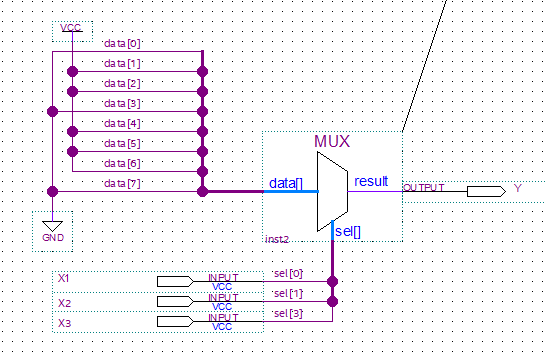
\includegraphics[width=0.6\linewidth]{img/dop3_sh}
	\caption{Условная схема подключения мультиплексора для функции \ref{eq:zad}}
	\label{fig:dop3_sh}
\end{figure}

\section{Контрольные вопросы}

\begin{enumerate}
	\item Каким логическим устройством (комбинационным/последовательностным) является	мультиплексор? Обоснуйте свой ответ.
	
	Мультиплексор является комбинационным устройством.
	Мультиплексор не хранит свое состояние, значение выходов зависит только от состояния входов.
	
	\item Приведите 3 примера реализации мультиплексора 4в1 на Verilog. Какая реализация лучше?

	Мультиплексор 4в1 можно реализовать оператором case, на основе тернарного оператора, использовать несколько мультиплексоров 2в1.
	
	Меньше всего пространства на чипе занимает мультиплексор на тернарном операторе.
	
	Самыми быстродействующими являются мультиплексор на операторе case и альтернативный модульный мультиплексор, в них по 2 параллельных мультиплексора.
	
	Лучше всего масштабируется по количеству информационных входов модульный мультиплексор.
	
	Лучше всего масштабируется по длине информационного сигнала альтернативный модульный мультиплексор.
	
	\item Что из себя представляет тестбенч при разработке на Verilog? Для чего требуется	разрабатывать тестбенчи?
	
	Тестбенчи -- специальные модули для тестирования и отладки схем и элементов на языке Verilog.
	
	\item В чем преимущества иерархического подхода при проектировании цифровых систем?
	
	При данном подходе сложные элементы создаются на основе простых.
	Данный подход позволяет упростить разработку сложных схем.
	
	\item Каковы преимущества подхода к проектированию мультиплексоров с использованием оператора case?
	
	Мультиплексор на операторе case явно задает состояние выходов при определенном входе.
	Кроме того, данный тип мультиплексоров обладает повышенным быстродействием
	
	\item Для чего используется ключевое слово default совместно с оператором case? Какие могут возникнуть проблемы при использовании директивы // synopsys full\_case parallel\_case?
	
	Ключевое слово default позволяет задать неопределенный уровень при подаче запрещенного сигнала.
	
	При использовании директивы synopsys full\_case parallel\_case схема может стать больше, медленнее;
	некоторые защелки могут исчезнуть
	
	\item Какую функцию выполняет демультиплексор? Приведите пример параметризируемого демультиплексора на Verilog.
	
	Демультиплексор выполняет обратную задачу мультиплексора -- подает на один из выходов входной сигнал.
	
	\VerbatimInput{../z1/bn_demux_1_4_case.v}
	
	\item Какова особенность селектора и в чем его отличие от мультиплексора?
	
	В селекторе адресный код декодирован в унитарный код.
	
	\item Для чего используется конструкция generate? Приведите пример.
	
	Конструкция generate нужна для создания однотипных блоков схем.
	Конструкция повышает читаемость и удобство проектирования.
	
	\item Для чего используется оператор частичного выбора (part select)? Приведите примеры.
	
	Данный оператор позволяет сокращенно записывать выражения с выбором определенных индексов у сигналов.
	
	\item Что такое распределенный селектор, и в каких задачах он может применяться? Приведите примеры.
	
	Распределенный селектор позволяет выбирать из множества сигналов, при чем данный селектор может обрабатывать данные не сразу все, а в некотором порядке.
	Это позволяет ускорять работу высокочастотных устройств, например процессоров.
	
\end{enumerate}

\section{Выводы по работе}

В ходе работы получен опыт проектирования схем в программе Quartus с помощью языка Verilog.
%Полученное устройство было протестировано с помощью бенчтестов в программе Quartus Simulation Waveform editor и ModelSim.
В процессе работы были смоделированы и получены RTL схемы  различных мультиплексоров, демультиплексоров и селекторов.
%В процессе работы были смоделированы различные шифраторы и дешифраторы, протестированы способы оптимизации схемы, а так же рассчитаны временные параметры схемы с различными способами оптимизации.
В процессе был получен опыт работы с платой DE10-Lite, на которой проверялась работоспособность полученного устройства.

\newpage 
\renewcommand{\refname}{{\normalsize Список использованных источников}} 
\centering 
\begin{thebibliography}{9} 
	\addcontentsline{toc}{section}{\refname} 
	\bibitem{Verilog} Thomas D., Moorby P. The Verilog Hardware Description Language. – Springer Science \& Business Media, 2008.
	\bibitem{citekey} Khor W. Y. et al. Evaluation of FPGA Based QSPI Flash Access Using Partial Reconfiguration //2019 7th International Conference on Smart Computing \& Communications (ICSCC). – IEEE, 2019. – С. 1-5
\end{thebibliography}

\end{document} % конец документа






